\subsection*{Problema 16}

\textbf{Enunciado:} Evaluar la integral definida 
mediante sumas de Riemann usando una partición geométrica:
\begin{align*}
\int_{a}^{b} x^{-2} \, dx, \quad 0 < a < b
\end{align*}

\textbf{Solución:} Para resolver la integral 
utilizando una partición geométrica, 
definimos los puntos de la partición como:
\begin{align*}
x_i = a \left(\frac{b}{a}\right)^{i/n}, \quad i = 0, 1, 2, \dots, n
\end{align*}

La longitud del $i$-ésimo subintervalo 
$\Delta x_i = x_i - x_{i-1}$ es:
\begin{align*}
\Delta x_i &= a \left(\frac{b}{a}\right)^{i/n} 
- a \left(\frac{b}{a}\right)^{(i-1)/n} \\
&= a \left(\frac{b}{a}\right)^{(i-1)/n} 
\left[ \left(\frac{b}{a}\right)^{1/n} - 1 \right]
\end{align*}

Evaluamos la función $f(x) = x^{-2}$ 
en el extremo derecho del subintervalo, $x_i$:
\begin{align*}
f(x_i) &= \left[ a \left(\frac{b}{a}\right)^{i/n} \right]^{-2} \\
&= a^{-2} \left(\frac{b}{a}\right)^{-2i/n}
\end{align*}

Planteamos la suma de Riemann $S_n$:
\begin{align*}
S_n &= \sum_{i=1}^{n} f(x_i) \Delta x_i \\
&= \sum_{i=1}^{n} \left[ a^{-2} \left(\frac{b}{a}\right)^{-2i/n} \right] \\
&\quad \cdot a \left(\frac{b}{a}\right)^{(i-1)/n} 
\left[ \left(\frac{b}{a}\right)^{1/n} - 1 \right]
\end{align*}

Simplificando los términos exponenciales:
\begin{align*}
S_n &= \frac{1}{a} \left[ \left(\frac{b}{a}\right)^{1/n} - 1 \right] \\
&\quad \cdot \sum_{i=1}^{n} \left(\frac{b}{a}\right)^{-(i+1)/n}
\end{align*}

La suma restante es una progresión geométrica 
de razón $r = (b/a)^{-1/n}$:
\begin{align*}
S_n &= \frac{1}{a} \left[ \left(\frac{b}{a}\right)^{1/n} - 1 \right] \\
&\quad \cdot \left(\frac{b}{a}\right)^{-2/n} 
\frac{1 - \left(\frac{b}{a}\right)^{-1}}{1 - \left(\frac{b}{a}\right)^{-1/n}}
\end{align*}

Tomando el límite cuando $n \to \infty$, 
haciendo el cambio $u = 1/n$ y aplicando L'Hôpital:
\begin{align*}
\lim_{n \to \infty} S_n &= \frac{1 - \frac{a}{b}}{a \ln(b/a)} \cdot \left(\frac{b}{a}\right)^{-1} \\
&= \frac{b - a}{ab} \cdot \frac{1}{\ln(b) - \ln(a)} \\
&= \left[ -\frac{1}{x} \right]_{a}^{b} = \frac{1}{a} - \frac{1}{b}
\end{align*}

\begin{figure}[H]
	\centering
	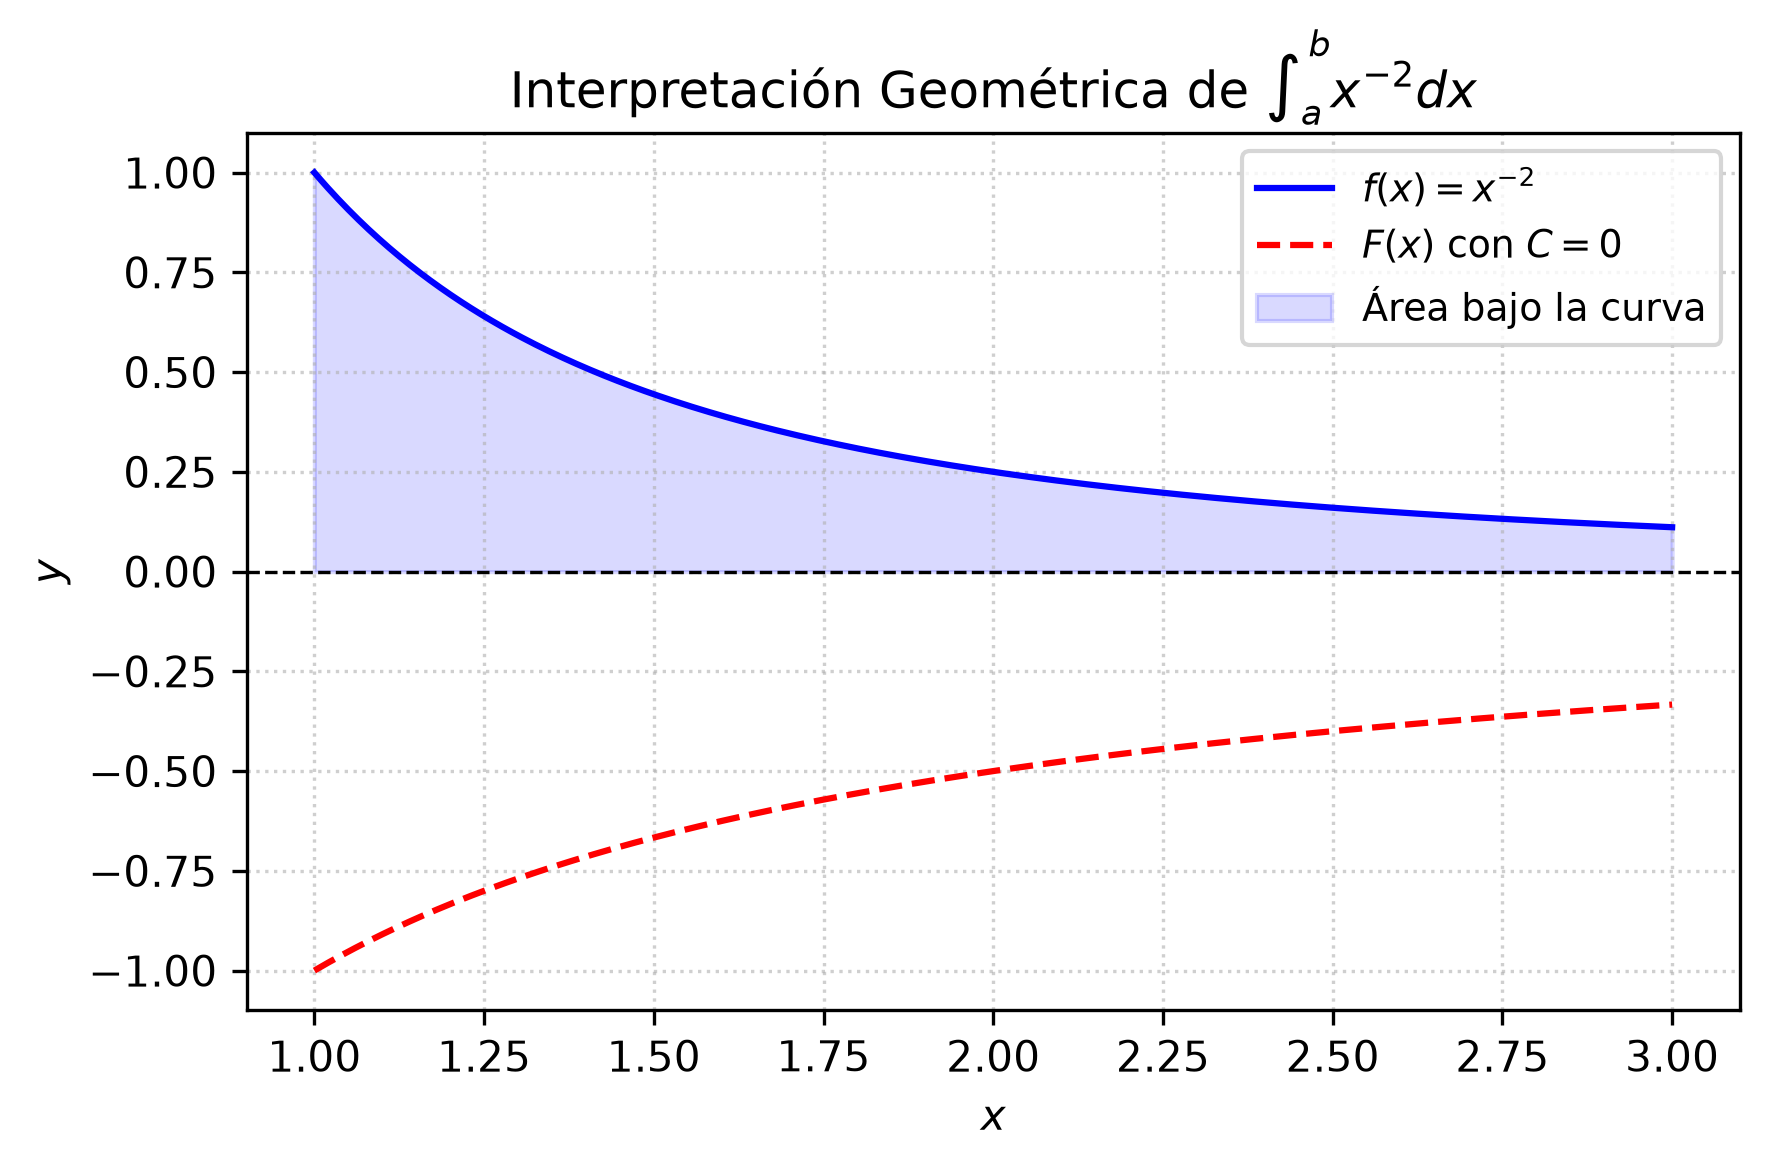
\includegraphics[width=\columnwidth]{semana_06/graficas/SEM06_P16_grafica.png}
	\caption{Representación gráfica de $f(x)$ y su antiderivada $F(x)$ evaluada para la constante de integración $C = 0$ (Problema 16).}
	\label{fig:problema16}
\end{figure}
